%%%%%%%%%%%%%%%%%%%%%%%%%%%%%%%%%%%%%%%%%%%%%%%%%%%%%%%%%%%%%%%%%%%%%%%%%%%%%%%
%                                                                             %
% 01 - Introducción y objetivos                                               %
%                                                                             %
%%%%%%%%%%%%%%%%%%%%%%%%%%%%%%%%%%%%%%%%%%%%%%%%%%%%%%%%%%%%%%%%%%%%%%%%%%%%%%%

\chapter{\textcolor{azulescom}{Introducción}}

La industria inmobiliaria en la actualidad enfrenta grandes desafíos en la
valuación de bienes inmuebles, donde la precisión y la eficiencia son cruciales
para el éxito de las transacciones \cite{pagourtzi2003}. Los profesionales
del sector y los inversionistas a menudo encuentran dificultades para determinar
los precios más apropiados de cada inmueble debido a la falta de herramientas
eficientes y la complejidad del mercado inmobiliario \cite{nedovic2000}.
La propuesta de este trabajo terminal implica el uso de nuevas tecnologías que
le ofrezcan al usuario la posibilidad de obtener un precio de mercado.

La inteligencia artificial ha demostrado un gran potencial en el análisis y la
toma de decisiones en diversos campos de alto impacto en nuestra sociedad como
lo son la medicina, la construcción, las finanzas, el comercio electrónico y el
sector inmobiliario \cite{pagourtzi2003}. Algunas investigaciones han
propuesto el uso de técnicas de inteligencia artificial, como el aprendizaje
automático y las redes neuronales, para mejorar la cobertura geográfica en la
estimación de valores de propiedades \cite{worzala1995,limsombunchai2004}.
La valuación de bienes inmuebles requiere la consideración de múltiples factores,
como la ubicación, las características de la propiedad, las tendencias del mercado
y las condiciones económicas \cite{limsombunchai2004}. Estos factores hacen que la
valuación de propiedades sea una tarea compleja y desafiante, que podría beneficiarse
del uso de técnicas avanzadas de inteligencia artificial para analizar la información
y generar estimaciones precisas.

En este contexto, se han comparado múltiples algoritmos y metodologías de
aprendizaje automático, cómo Extra Trees (ET), k–Nearest Neighbors (KNN), y
Random Forest (RF), dónde se observa que cada mercado cuenta con características
específicas que requieren incluirse en el proceso de estimación y por lo tanto
deben considerarse para lograr mejores resultados \cite{choy2023}.
Sin embargo, el planteamiento fundamental puede ser adaptado fácilmente en función
de la cobertura geográfica deseada.

La propuesta del presente Trabajo Terminal se enfoca en el desarrollo de un
método de estimación de costo para departamentos que, mediante el uso de
Inteligencia Artificial, sea capaz de realizar estimaciones de costo útiles
para un precio de mercado en la Ciudad de México a manera de facilitar y
optimizar el tiempo que toma obtener un vistazo inicial a lo que podría ser el
valor del inmueble en cuestión.

Actualmente, en el mercado se encuentran algunas soluciones que hacen uso de
inteligencia artificial para la valuación de propiedades,
como Zillow's Zestimate \cite{zillow2023} y HouseCanary \cite{housecanary2021}.
Sin embargo, estas soluciones aún presentan limitaciones en términos de cobertura
y adaptabilidad a diferentes
mercados y contextos. La propuesta busca abordar estas limitaciones y ofrecer
una herramienta más adaptable al mercado mexicano, más específicamente al de la
Ciudad de México.

\section{Estado del Arte}
A continuación, se presenta el Cuadro \ref{table:PropuestasSimilares} con las
características de aplicaciones web similares y comparándolos con la propuesta.
Dentro de las características se incluye el tipo de aplicación, las características
de estimación de costo, la cobertura geográfica y el precio en el mercado.

\begin{table}[H]
    \caption[Resumen de productos similares]{Resumen de productos similares comparados con la propuesta}
    \centering
    \begin{tabular}{|m{3.5cm}|m{6.5cm}|m{3.5cm}|}
        \hline
          \rowcolor{azulclaro}
          \multicolumn{1}{|c|}{\textbf{Software}} &
          \multicolumn{1}{c|}{\textbf{Características}} &
          \multicolumn{1}{c|}{\textbf{Precio en el mercado}} \\
        \hline
        Zillow’s Zestimate \cite{zillow2023} & Aplicación web que ofrece una estimación de costo de bienes inmobiliarios, hace uso de inteligencia artificial para obtener los valores de cada característica, los datos usados son los propios de Zillow (marketplace de bienes raíces) permite ingresar detalles específicos a cada tipo de inmueble y ofrece una valuación muy precisa y detallada, sin embargo solo tiene cobertura en el mercado de EE.UU. y Canadá. & Gratuito \\
        \hline
        House Canary \cite{housecanary2021} & Aplicación web que ofrece una estimación de costo de bienes inmobiliarios, hace uso de inteligencia artificial para obtener las estimaciones de cada característica, permite ingresar detalles específicos a cada inmueble, sólo tiene cobertura en EE.UU. y Canadá. & Considerando el producto \textit{Agile Evaluation}, \$ 0.80 USD por valuación  \\
        \hline
        Estimador de costo de Inmuebles24 \cite{inmuebles24} & Aplicación web que ofrece una estimación aproximada de costo para bienes raíces, hace uso de inteligencia artificial para obtener la estimación de costo general, los datos utilizados son de su propio sitio web (marketplace de bienes raíces), su cobertura es baja y únicamente entrega el precio de mercado. & Gratuito \\
        \hline
        Propuesta de herramienta en el presente trabajo terminal & Aplicación web que ofrecerá una estimación aproximada de costo para departamentos en la Ciudad de México, hace uso de inteligencia artificial para obtener la estimación de costo general, la cobertura será determinada por la disponibilidad del conjunto de datos a emplear. & Gratuito \\
        \hline
    \end{tabular}
    \label{table:PropuestasSimilares}
\end{table}

\section{Objetivos}

\subsection{Objetivo general}

Crear una herramienta de apoyo para profesionales del sector inmobiliario,
inversionistas o cualquier persona interesada en la estimación de costo de algún
departamento en la Ciudad de México para que puedan obtener un precio de mercado.

Mediante el uso de un conjunto de datos (\gls{dataset}) y servicios de la nube (Amazon
Web Services) los datos se procesarán a fin de crear un módulo que pueda identificar
patrones a través de redes neuronales para ofrecer un estimado de precio a partir
de un conjunto de características que clasifiquen al inmueble. A su vez, se
desarrollará una interfaz web intuitiva a modo de prototipo con el fin de que el
usuario pueda visualizar el estimado de precio del inmueble en cuestión.

Dicha herramienta pretende ayudar a los usuarios descritos con el fin de que
puedan obtener una estimación de costo que les permita tener un aproximado de
precio de mercado.

\subsection{Objetivos particulares}

\begin{itemize}
  \item Generar un conjunto de datos (\gls{dataset}) con precios históricos de bienes
  inmobiliarios en la Ciudad de México para efecto de entrenamiento del modelo
  de aprendizaje automático.
  \item Hacer uso de alguna herramienta que utilice aprendizaje automático
  (machine learning) e implementar su uso en la nube para ayudar a procesar los
  anuncios de un tipo de inmueble particular.
  \item Desarrollar una interfaz web intuitiva a modo de prototipo que utilice
  una aplicación web alojada en infraestructura de nube para la captura de los
  datos del usuario así como la entrega de la estimación de precio calculada
  por el modelo.
\end{itemize}

\section{Justificación}

La generación de estimaciones precisas y eficientes para la valuación de bienes
inmuebles puede ser un desafío abrumador para profesionales y aficionados, debido
a la falta de herramientas adecuadas y la complejidad del mercado inmobiliario.
En ocasiones, se pueden recurrir a servicios especializados en la valuación de
propiedades, pero estos pueden resultar costosos y no siempre cumplir con las
expectativas del usuario. Por tanto, este trabajo terminal busca desarrollar una
herramienta que facilite el proceso de estimación de costos para departamentos
en la Ciudad de México, beneficiando a profesionales del sector inmobiliario,
inversionistas e interesados en general en el sector inmobiliario.

Por lo general, la valuación de bienes inmuebles implica la consideración de
múltiples factores, como la ubicación, las características de la propiedad y
las tendencias del mercado \cite{limsombunchai2004}. Estos patrones pueden ser
identificados mediante el uso de inteligencia artificial y el análisis de datos
históricos y actuales del mercado inmobiliario. Al enfocar el análisis en el
mercado de la Ciudad de México, se espera que el modelo propuesto sea más
relevante y preciso para este contexto específico.

El trabajo terminal propone utilizar técnicas avanzadas de inteligencia artificial,
como el aprendizaje automático y las redes neuronales, para mejorar la cobertura
en la estimación de costos de departamentos en la Ciudad de México \cite{worzala1995}.
Además, se plantea implementar la solución en un entorno en la nube, lo que
facilitaría la adaptación y flexibilidad de la plataforma, permitiendo su
actualización y mantenimiento independientemente de la implementación.

A diferencia de las soluciones existentes en el mercado, como Zillow's Zestimate
y HouseCanary, este proyecto busca desarrollar un método de estimación de costo
específicamente adaptado al mercado inmobiliario de la Ciudad de México, utilizando
tecnologías y enfoques diferentes para lograr resultados más precisos y relevantes
\cite{housecanary2021,zillow2023}.

Se utilizarán conocimientos adquiridos durante la carrera para llevar a cabo un
análisis eficaz y detallado de la problemática y las opciones de solución. Para
ello, se retomarán técnicas de gestión y diseño de proyectos vistas en
\textit{Administración de Proyectos}, \textit{Gestión Empresarial} e
\textit{Ingeniería de Software}, conocimientos de programación como en
\textit{Programación Orientada a Objetos}, \textit{Sistemas Distribuídos} y
\textit{Desarrollo Web}, técnicas de \textit{Inteligencia Artificial} y
\textit{Análisis de Datos} y, finalmente, se hará uso de herramientas de
comunicación y redacción científica vistas en \textit{Comunicación Oral y Escrita}
para un análisis detallado del ámbito de la valuación inmobiliaria permitiendo un
detallado y eficaz análisis del problema y las soluciones disponibles.

\section{Metodología}

Para el desarrollo de este trabajo terminal se optó por la metodología ágil SCRUM,
debido a que, como proceso de gestión de proyectos, se reduce complejidad y
permite actuar rápidamente ante cualquier cambio para poder satisfacer las
necesidades de los clientes. Una de las cualidades más importantes de SCRUM
es que nos ofrece una clara visibilidad sobre el avance del proyecto así como de
los pasos intermedios a realizar en cada sprint para alcanzar los objetivos. Además,
permite trabajar de manera eficiente colaborativamente, es decir, en equipo,
para obtener el mejor resultado posible.

Ken Schwaber y Jeff Sutherland \cite{schwaber2016} explican Scrum de una manera clara y simple.
Dicen que no es una colección de partes y/o componentes definidos de manera
prescriptiva, sino que está basado en un modelo de proceso empírico, basado en
la autoorganización de los equipos los cuales logran lidiar con lo imprevisible,
resolviendo los problemas complejos inspeccionándolos y adaptándose continuamente.

SCRUM contiene los siguientes eventos:

\begin{itemize}
  \item \textbf{Sprint Planning}: Reunión de planificación del sprint, en la que
  el equipo de desarrollo selecciona las tareas que se van a realizar durante el
  sprint.
  \item \textbf{Daily Scrum}: Reunión diaria de seguimiento, en la que el equipo
  de desarrollo se sincroniza sobre el estado de las tareas.
  \item \textbf{Sprint Review}: Reunión de revisión del sprint, en la que el
  equipo de desarrollo muestra los resultados del sprint.
  \item \textbf{Sprint Retrospective}: Reunión de retrospectiva del sprint, en
  la que el equipo de desarrollo analiza el sprint y propone mejoras.
\end{itemize}

Estos eventos existen con el fin de establecer una regularidad y minimizar la
necesidad de reuniones no definidas en Scrum. Estos eventos son bloques de
tiempo (\textit{time boxes}), de tal forma que todos cuentan con una duración máxima.

También se definen los siguientes artefactos:

\begin{itemize}
  \item \textbf{Product Backlog}: Lista de requisitos del producto, ordenados
  por prioridad.
  \item \textbf{Sprint Backlog}: Lista de requisitos del producto seleccionados
  para el sprint actual.
  \item \textbf{Incremento}: Conjunto de requisitos del producto completados
  durante el sprint actual.
\end{itemize}

Los artefactos en SCRUM se definen para así fomentar la transparencia de la
información de tal manera que todos los involucrados tengan el mismo entendimiento
de que es lo que se está llevando a cabo, además de que facilita oportunidades
para realizar inspecciones y adaptaciones.

De igual manera, se pueden crear sprints, los cuales son ciclos breves de un mes
o menos con diferentes fases, en las cuales al final de cada ciclo se define la
fecha para la entrega de una versión del producto deseado. Debido a que se trata
de una versión, no se indica la finalización del proyecto, en otro caso que habrá
un mantenimiento constante para que se obtenga un producto final óptimo.

En virtud de que con el uso de SCRUM se logra la integración de todas las partes
involucradas en el proyecto, la administración y participación es sencilla y
fácil de manejar para todas las etapas. Asimismo, se cuenta con un registro de
las labores realizadas y se le da un seguimiento. De igual forma nos proporciona
una respuesta rápida a los cambios, así como la implementación de pruebas
funcionales durante el proceso.

\subsection{Implementación de la metodología}

Para la implementación de la metodología SCRUM se utilizará la herramienta
\textit{Trello} \cite{trello2023}, la cual es una aplicación web que permite
organizar proyectos en tableros. En cada tablero se pueden crear listas, las
cuales pueden contener tarjetas, las cuales a su vez pueden contener listas de
chequeo, etiquetas, fechas de vencimiento, archivos adjuntos, entre otras
características. En la Figura \ref{fig:trello} se muestra un ejemplo de un
tablero de \textit{Trello}.

\begin{figure}[!htbp]
  \centering
  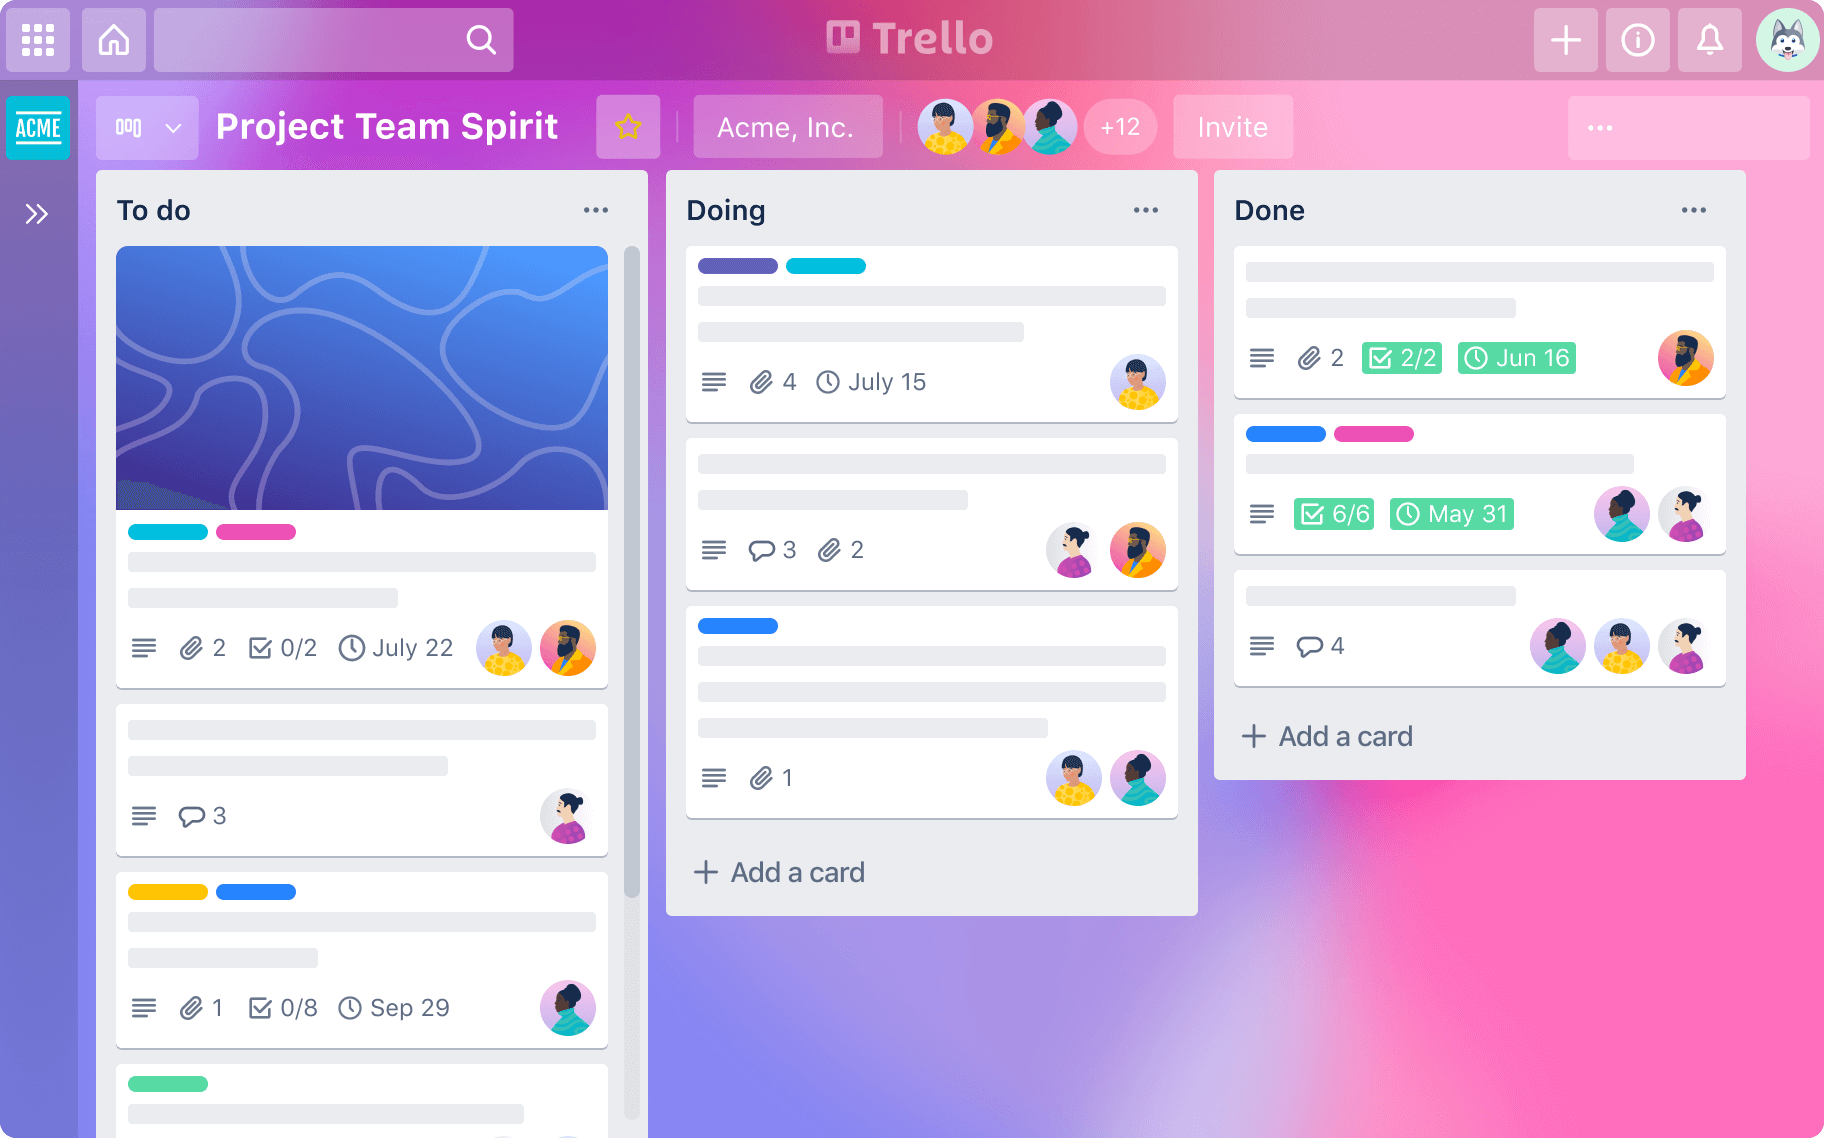
\includegraphics[width=0.9\textwidth]{imagenes/01-introduccion/trello-board.png}
  \caption[Ejemplo de un tablero de Trello]{Ejemplo de un tablero de Trello \cite{trello2023}}
  \label{fig:trello}
\end{figure}

Para implementar la metodología SCRUM en \textit{Trello}, se creará un tablero
para el proyecto, en el cual se crearán las siguientes listas:

\begin{itemize}
  \item \textbf{Product Backlog}: Lista de requisitos del producto, ordenados
  por prioridad.
  \item \textbf{Sprint Backlog}: Lista de requisitos del producto seleccionados
  para el sprint actual.
  \item \textbf{Sprint}: Lista de tareas que se realizarán durante el sprint
  actual.
  \item \textbf{Done}: Lista de tareas que se han completado.
\end{itemize}

En la Figura \ref{fig:trello_scrum} se muestra un ejemplo de un tablero de
\textit{Trello} con las listas descritas anteriormente.

\begin{figure}[!htbp]
  \centering
  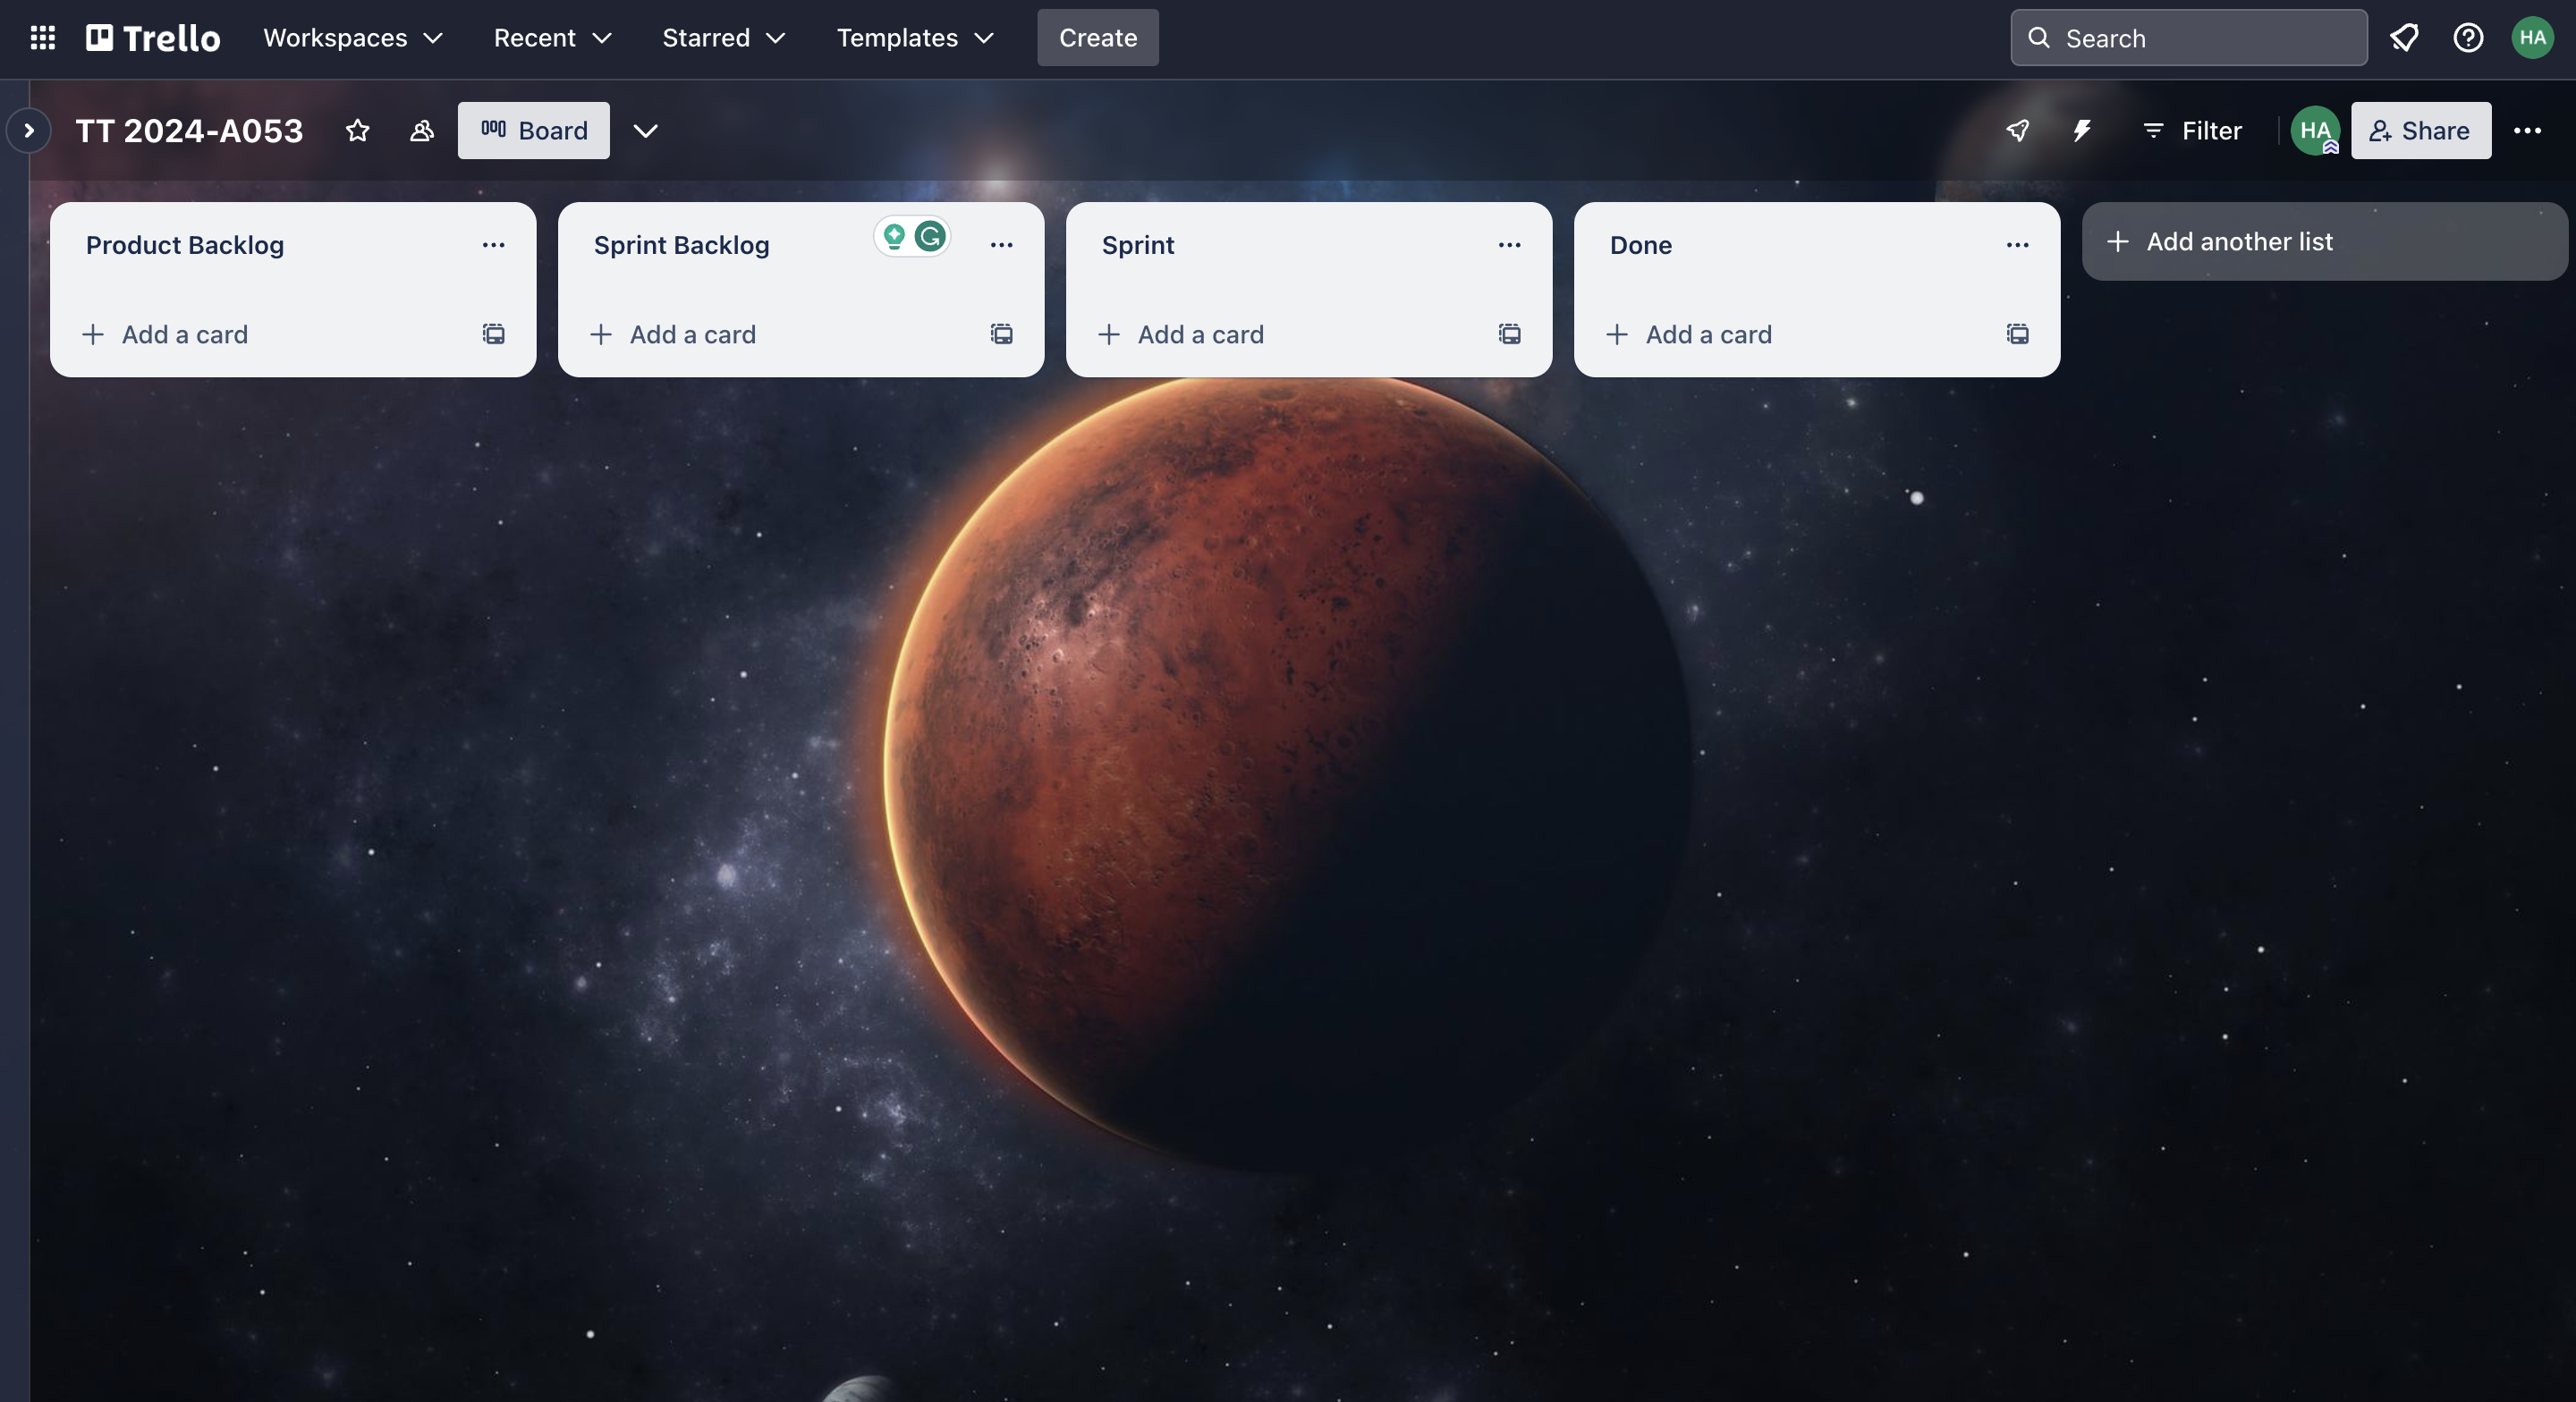
\includegraphics[width=0.9\textwidth]{imagenes/01-introduccion/trello-scrum.png}
  \caption[Ejemplo de un tablero de Trello con la metodología SCRUM]{Ejemplo de un tablero de Trello con la metodología SCRUM}
  \label{fig:trello_scrum}
\end{figure}

La intención será que cada tarjeta en la lista \textit{Product Backlog} represente
una tarea, la cual se moverá a la lista \textit{Sprint Backlog} cuando se decida
que se realizará en el sprint actual. Posteriormente, cada tarea se dividirá en
subtareas, las cuales se agregarán a la lista \textit{Sprint}. Finalmente, cuando
se complete una subtarea, se moverá a la lista \textit{Done}.

\subsection{Iteraciones (Sprints)}

Para la implementación de la metodología SCRUM se realizarán iteraciones (o
sprints) de una duración de 2 semanas, las cuales se llevarán a cabo a lo largo
del desarrollo del presente trabajo terminal.

\subsubsection{Trabajo Terminal I}

\begin{itemize}
  \item Construir una base de datos de anuncios de bienes inmuebles en la Ciudad
  de México, la cual contendrá las características fundamentales de cada anuncio,
  así como su precio de venta.
  \item Realizar una limpieza a los datos extraídos del \gls{dataset}.
  \item Realizar un análisis exploratorio de datos para identificar patrones
  relevantes en los datos.
\item Seleccionar los algoritmos de aprendizaje automático que mejor se adapten
  a los datos.
  \item Seleccionar las herramientas necesarias para trabajar en
  la construcción de un modelo utilizando redes neuronales.
\end{itemize}

\subsubsection{Trabajo Terminal II}

\begin{itemize}
  \item Generar un modelo en la nube para su entrenamiento utilizando las redes
  neuronales previamente elegidas.
  \item Implementar la interfaz que el usuario final verá.
  \item Integrar la interfaz con la aplicación que utiliza el modelo utilizando
  un servidor web.
  \item Realizar las pruebas pertinentes, así como la reingeniería requerida.
  \item Desarrollar el manual técnico y el de usuario.
\end{itemize}

\section{Organización del documento}

A manera de que el lector pueda tener un entendimiento más claro de la estructura
de este documento, se presenta a continuación una breve descripción de cada uno
de los capítulos que lo conforman.

\subsection*{Capítulo 2. Marco teórico}

La sección de \textit{Marco teórico} se divide en dos partes, la primera parte
se enfoca en la descripción del contexto en el que se desarrolla el trabajo
terminal, es decir, se habla de la industria inmobiliaria y la valuación de
bienes inmuebles, así como la importancia de la inteligencia artificial en este
sector. La segunda parte se enfoca en la descripción de los conceptos teóricos
que se utilizarán a lo largo del trabajo terminal, es decir, se habla de las
redes neuronales, el aprendizaje automático y las herramientas que se utilizarán
para el desarrollo del trabajo terminal.

\subsection*{Capítulo 3. Análisis}

En el tercer capítulo, se describe el análisis realizado para la elaboración de
este trabajo terminal.

Para esto, se divide en tres secciones, la primera sección se enfoca en la
descripción del problema, es decir, se habla de la problemática que se busca
resolver con este trabajo terminal, así como los objetivos que se pretenden
alcanzar y las delimitaciones que se tienen para este trabajo terminal.

La segunda sección se enfoca en la descripción de la propuesta, es decir, se
habla de la solución que se propone para resolver la problemática planteada,
así como los beneficios que se obtendrán al implementar esta solución.

La tercera sección se enfoca en la descripción de la factibilidad, es decir, se
habla de los recursos necesarios para la elaboración de este trabajo terminal,
así como las herramientas que se utilizarán para el desarrollo del mismo.

\subsection*{Capítulo 4. Diseño}

En el cuarto capítulo, se describe el diseño realizado para la elaboración de
este trabajo terminal.

Para esto, se divide en dos secciones, la primera sección se enfoca en la
descripción del diseño de la base de datos, es decir, se habla de la estructura
de la base de datos que se utilizará para el desarrollo de este trabajo terminal.

La segunda sección se enfoca en la descripción del diseño de la aplicación web,
es decir, se habla de la estructura de la aplicación web que se utilizará para
el desarrollo de este trabajo terminal.

\subsection*{Capítulo 5. Implementación}

En el quinto capítulo, se describe la implementación realizada para la elaboración
de este trabajo terminal. Se divide en: desarrollo de los modelos, desarrollo del
servicio web, desarrollo de la interfaz gráfica, despliegue en la nube, pruebas
del sistema y costos de operaación.

\subsection*{Capítulo 6. Conclusiones}

En el sexto capítulo, se presentan las conclusiones obtenidas a lo largo de la
realización de este trabajo terminal, incluyendo los resultados obtenidos y los
retos técnicos enfrentados.

\subsection*{Capítulo 7. Trabajo a futuro}

En el séptimo capítulo, se presentan las propuestas de trabajo a futuro para
continuar con el desarrollo de este trabajo terminal.

